% This file contains the content for a main section
\regularsectionformat
%% Modify below this line %%
\chapter{Conventions and Constraints}
\label{sec:conventions}

Some characteristics of the XML format are constrained to improve interoperability and interchange between the different systems that use LUTs. These constraints may be loosened over time as implementations and computer capabilities improve. It is desirable that implementations support the full capabilities of the specification, but it is recognized that portability and ease of implementation are needed in current deployments.

The constraints listed in this section serve to identify key parameters that an implementation reader must be able to use.

Among these agreed upon conventions are:

This specification uses the \texttt{ProcessList} as the root node in an XML file.  Storing multiple \texttt{ProcessList}s in a file requires definition of a higher-level XML schema for that purpose which is not addressed here.

Matrices are 3x3, 3x4, or 4x4. 3x4 matrices provide an offset value in the 4th column to be added to the results of the previous 3 columns.  

3-component processing is the normal mode of operation.  1-component processing is possible with only a \texttt{LUT1D} node and if needed a \texttt{Range} node, but is not a required feature.

\texttt{LUT3D}s have the same dimension on all axes (i.e. \texttt{Array} dimensions are of the form "n n n 3").  A \texttt{LUT3D} with axial dimensions greater than 128x128x128 should be avoided.

Software applications are required to support two 3DLUT interpolation types: ``trilinear'' and ``tetrahedral''.  ``Linear'' interpolation is required as a default for 1DLUTs.

\texttt{LUT1D} lengths should be limited to at most 65536 entries.

As a general principle, the LUT output values should make explicit the clipping behavior for values outside of the region of interest. The \texttt{Range} node can be used for clamping of values.

Supported bit depth values are ``\texttt{8i}'', ``\texttt{10i}'', ``\texttt{12i}'', ``\texttt{16i}'', ``\texttt{16f}'' and ``\texttt{32f}''.

``\texttt{12i}'' is present for processing of digital cinema 12-bit DCDMs. ``\texttt{16f}'' are half floats as described in IEEE 754-1985. All integer values are unsigned ints. ``\texttt{32f}'' LUTs should never be fully enumerated.
 
\begin{figure}[htbp]
\begin{center}
    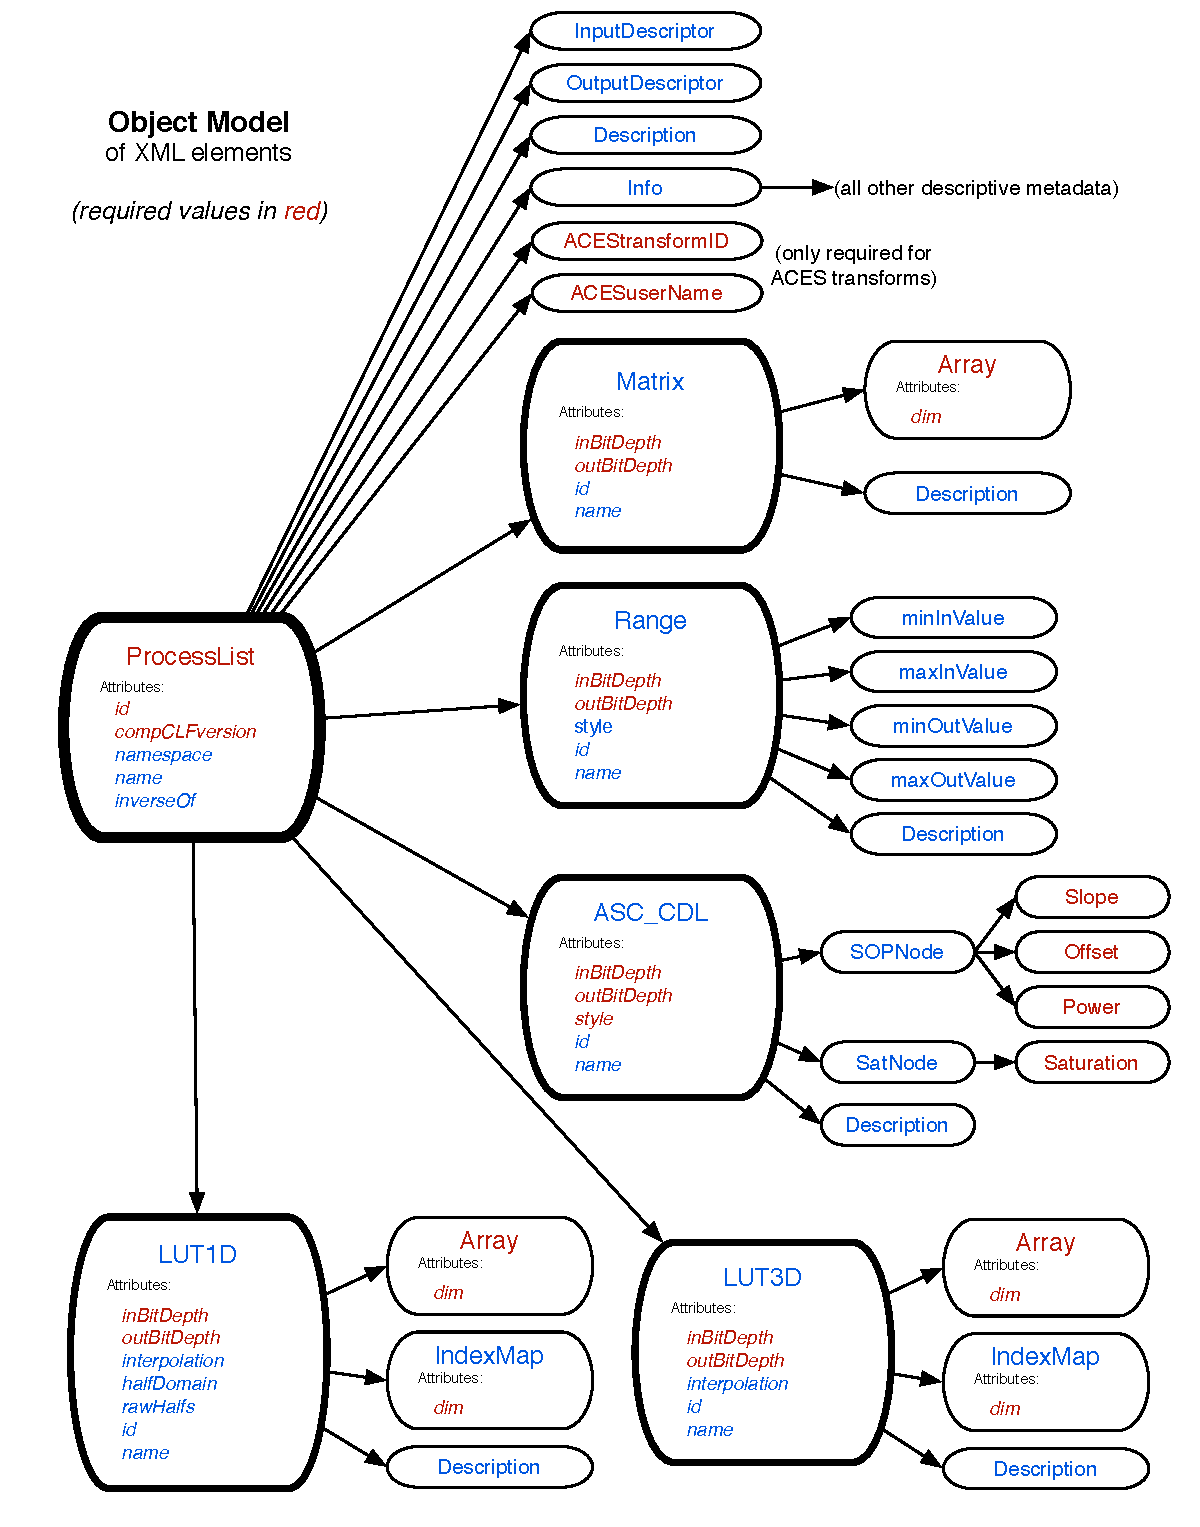
\includegraphics[width=\textwidth]{objectModel.pdf}
\caption{Object Model of XML Elements}
\label{fig:lmt}
\end{center}
\end{figure}